\subsection{Svelte}

% Kniha: https://www.syncfusion.com/succinctly-free-ebooks/svelte-succinctly
% https://vercel.com/docs/beginner-sveltekit
Svelte je relativně novým open-source JavaScript frameworkem, za jejímž stvořením stojí vývojář Richard Harris. 
Framework se odlišuje tím, že kompiluje komponenty přímo do čistého, nativního a~vysoce optimalizovaného JavaScriptu bez potřeby runtime. 
To vše ještě před tím, než uživatel navštíví webovou aplikaci v~prohlížeči. 
Tato metoda oproti klasickým deklarativním frameworkům, jako jsou např.~Angular, React či Vue, poskytuje výhodu především v~rychlosti. 
Technologie je určena k~vývoji kompaktního a~rychlého uživatelského rozhraní webových aplikací.\cite{sveltemdn,svelte,sveltedevinterface}

\begin{figure}[htb]
	\centering
		
\includegraphics[width=.3\textwidth]{images/svelte-logo.png}
	\caption[Svelte logo]{Svelte logo \cite{svelte}}
	\label{fig:sveltelogo}
\end{figure}

První verze byla představena ke konci roku~2016. Verze~3, jež byla vydána v~dubnu~2019, přinesla vylepšení týkající se zjednodušení tvorby komponent. 
Mimo jiné tato verze hlavně představila vylepšení ve smyslu reaktivity. Po této verzi framework nabral na popularitě díky jeho jednoduchosti.
Verze~4 pak v~roce~2023 představila pouze minimální změny, jež spočívají v~údržbě a~přípravách pro verzi nastávající.

Přestože Svelte nedisponuje rozsáhlým ekosystémem jako jiné JS frameworky, získal si přízeň mnoha velkých společností. 
Mezi ně patří například firmy jako The New York Times, Avast, Rakuten a~Razorpay.\cite{sveltemdn,svelte,sveltedevinterface}

\subsubsection{Komponenty}

Podobně jako v~jiných frameworcích, komponenty jsou základní stavební bloky Svelte. Komponentu tvoří HTML, CSS a~JavaScript, kde vše patří do jednoho souboru s~příponou .svelte. 
Všechny tři části komponenty jsou nepovinné. Logika komponenty musí být zapsána mezi párové script tagy. Následuje jedna nebo více značek pro definovaní šablony komponenty. 
V~neposlední řadě kaskádové styly se zapisují mezi značky style.

V~rámci šablony Svelte umožňuje využívat logické bloky pro podmíněné vykreslování nebe také iterace přes pole hodnot (list). 
Zabudovaná je i~podpora manipulace s~asynchronním JavaScriptem - promises.\cite{svelte}

\begin{prog}
<script>
  let content = 'nějaký-obsah';
</script>

<div>\{content\}</div>
  
<style>
  div \{
    background-color: red;
  \}
</style>
\end{prog}

\subsubsection{Reaktivita}

Srdcem Svelte jsou reaktivní stavy komponenty, které jednoduše definujeme jako proměnné v~JavaScriptu. Jejich hodnotu aktualizuje JS funkce pomocí přidělování nových hodnot. 
Kupříkladu stav datového typu pole nelze aktualizovat pomocí metody push či splice. Je nutné využít jiné intuitivní řešení pomocí přidělení nové hodnoty.
O~vše ostatní se pak postará samotný framework. Svelte aktualizuje DOM při každé změně stavu komponenty. 

Mezi specifické funkce Svelte patří reaktivní deklarace, které se starají o~aktualizaci stavů na základě stavů jiných. 
Další zabudovanou funkcí jsou tzv. reactive statements, jež umožní definovat akce, které se mají vykonat reaktivně -- jako reakce na nějaký výrok.\cite{sveltehandbook,svelte}

\begin{prog}
<script>
  let count = 0;

  function increment() \{
    count++;
  \}
</script>

<button on:click=\{increment\}>
  Klikli jste na tlačítko \{count\}x.
</button>
\end{prog}

\subsubsection{Předávání vlastností}

Pro komunikaci mezi komponentami slouží mechanismus předávání vlastností. 
K~předání vlastnosti do vnořené komponenty využijeme HTML atribut, pomocí kterého získáme danou hodnotu ve vnořené komponentě.  
Uvnitř vnořené komponenty vytvoříme stejnojmennou vlastnost s~klíčovým slovem export.

V~případě, že chceme předávat aktualizovanou vlastnost z~vnořené do rodičovské komponenty, je třeba vytvořit vlastnost již na rodiči. 
Následně ji předáme vnořené komponentě pomocí bind direktivy. Bind zajistí aktualizaci hodnoty stavu i~v~rodičovké komponentě.\cite{svelte}

\begin{prog}
// Parent.svelte
<script>
  import ChildComponent from './Child.svelte';

  const someProps = \{color: 'cervena'\};
</script>

<ChildComponent color='cervena' />
<ChildComponent color=\{someProps.color\} />
<ChildComponent \{...someProps\} />

// Child.svelte
<script>
  export let color;
</script>

<div class=\{color\}></div>
\end{prog}

\subsubsection{Eventy} % Přidat actions

Svelte má velice jednoduché API pro práci s~DOM událostmi (eventy). Na element stačí přidat direktivu on s~názvem eventu. 
Následně předáme callback funkci, v~níž provedeme požadovanou akci.

\begin{prog}
<script>
  let count = 0;
</script>

<button on:click=\{() => count++\}>
  Klikli jste na tlačítko \{count\}x.
</button>
\end{prog}

Vývojáři také přišli s~možností odesílání a~přijímání eventů pro komponenty. 
Uvnitř vnořené komponenty je třeba mít DOM event handler, na který chceme reagovat v~rodičovské komponentě. 
Poté je nutné využít zabudovanou funkci createEventDispatcher, které předáme potřebné parametry -- libovolný název pro event komponenty a~hodnotu. 
V~rodičovské komponentě pak reagujeme na event pomocí klíčového slova on a~našeho libovolného názvu pro event. Hodnotu poté získáme v~callback funkci.\cite{sveltehandbook,svelte}

\begin{prog}
// Parent.svelte
<script>
  import Child from './Child.svelte';

  function handleMessage(event) \{
    alert(event.detail.text);
  \}
</script>

<Child on:message=\{handleMessage\} />

// Child.svelte
<script>
  import \{ createEventDispatcher \} from 'svelte';

  const dispatch = createEventDispatcher();

  function sayHello() \{
    dispatch('message', \{
      text: 'Hello world!'
    \});
  \}
</script>

<button on:click=\{sayHello\}>Klikněte pro "Hello world!"</button>
\end{prog}

Zdroj zdrojového kódu: \cite{svelte}

\subsubsection{Životní cyklus}

Komponenty ve Svelte disponují životním cyklem, který začíná v~momentě vytvoření komponenty a~končí jejím zničením. 
Funkce onMount tvoří callback, který je zavolán po přidání komponenty do DOM. Pokud chceme vykonat určité akce při zničení komponenty, můžeme toho dosáhnout dvěma způsoby. 
Prvním způsobem je vracení callback funkce v~rámci onMount funkce. Druhou možnost představuje využití funkce onDestroy, která v~argumentu přijímá callback funkci. 

Pro práci převážně s~imperativními akcemi slouží zabudované funkce beforeUpdate a~afterUpdate. 
V~případě beforeUpdate funkce jde o~callback, který se volá před aktualizací komponenty, tj. před prvním voláním onMount nebo po každé změně stavu. 
Oproti tomu, afterUpdate je callbackem, jenž Svelte vykoná po prvním zavolání onMount nebo po každé aktualizaci komponenty.\cite{sveltehandbook,svelte}

\begin{figure}[htb]
	\centering
		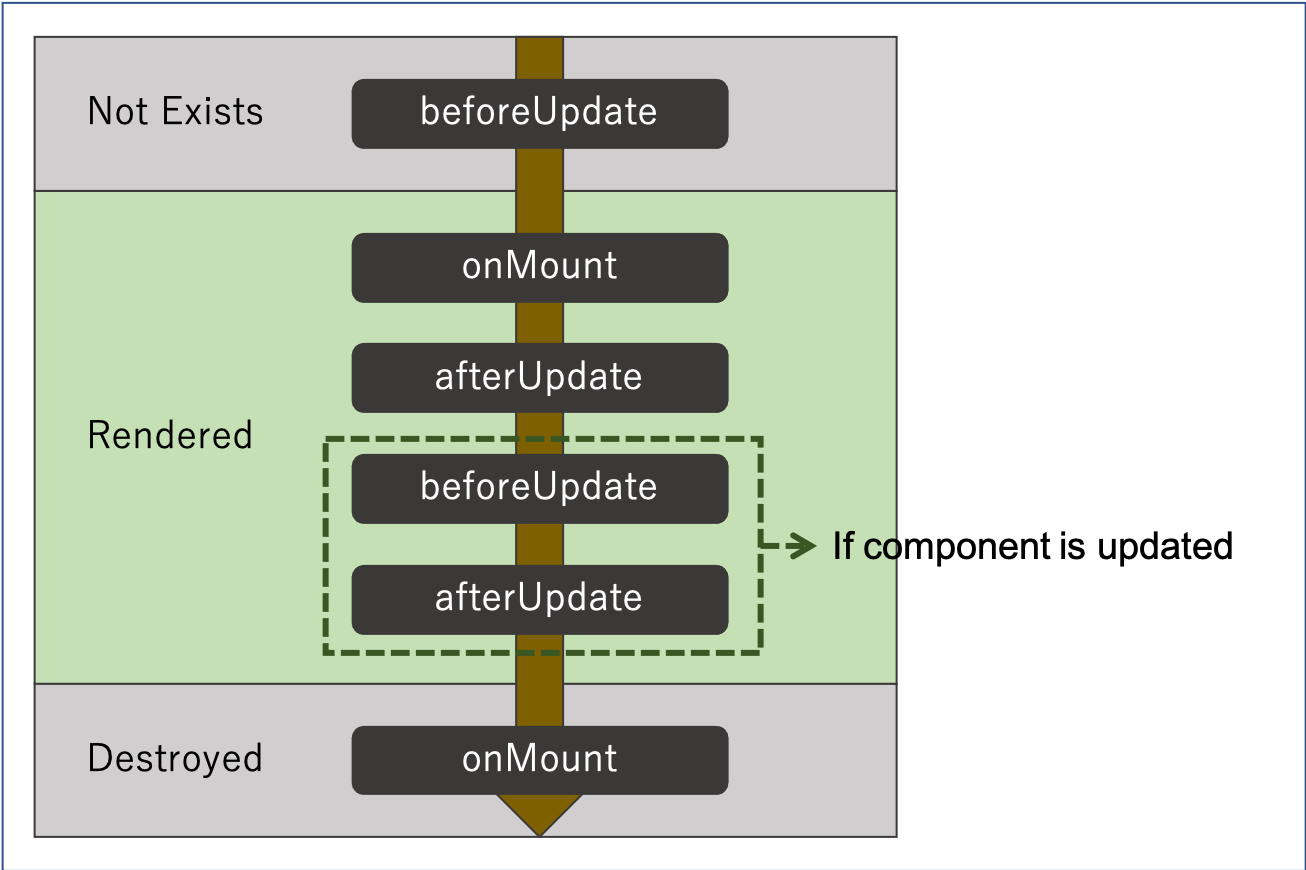
\includegraphics[width=.8\textwidth]{images/sveltelifecycle.png}
	\caption[Životní cyklus Svelte]{Životní cyklus Svelte \cite{sveltelifecycle}}
	\label{fig:sveltelifecycle}
\end{figure}

\subsubsection{State management}

Svelte poskytuje pestrou škálu API pro správu stavů aplikace v~závislosti na rozsahu a~složitosti ukládaných dat. 
Základním přístupem pro správu stavů je ukládání a~manipulace se stavy v~rámci stromu komponent. 
To zahranuje tvorbu reaktivních stavů a~jejich distribuci ve stromě pomocí předávání vlastností, bindování či eventů. 

Další možnost představuje využití Context API, které umožňuje jednorázové uložení jakékoli hodnoty. 
Hodnotu uloženou v~kontextu můžeme získat i~v~rámci neincidentních komponent. Ukládání a~získávání kontextu umožňují funkce setContext a~getContext.

Pro sofistikovanější práci se stavy slouží tzv. stores. V~podstatě se jedná o~globání úložiště stavů, které umožňuje uchovávat a~získávat data. 
Store je jednoduše objekt s~metodou subscribe, která umožní konzumentům dostat aktualizovaná data. 
Jednodušší variantu pro získání aktuálních dat představuje použití znaku \$ před názvem proměnné. Svelte nám poskytuje hned několik podob storu. 
Mezi ně patří writable a~readable stores, kde jediný rozdíl spočívá v~možnosti aktualizace dat. 
Pro stavy, které jsou odvozeny z~jiných stores, existuje tzv. derived store. Svelte rovněž povoluje vytvořit i~vlastní store. 
% Store je možné používat i v klasických JS filech, např pomocí subscribe... 

Již zabudované globální úložiště můžeme jednoduše vytvořit pomocí metod writable, readable a~derived. Writable požaduje jako argument počáteční hodnotu. 
Readable navíc jako druhý argument může přijímat funkci start, jež implementuje callbacky volající se při prvním a~posledním subscribe.\cite{sveltehandbook,svelte,sveltestatemanagement}

\subsubsection{Routování}

Svelte nemá přímou podporu routování v~aplikacích. Oficiální dokumentace uvádí jako oficiální knihovnu pro routování SvelteKit. 
Ve skutečnosti se jedná o~framework nad Svelte, který poskytuje i~další možnosti rozšíření webové aplikace. 
Dokumentace však doporučuje i~jiné knihovny pro routování na základě odlišných přístupů. 
Konkrétně knihovny page.js, svelte-routing, svelte-navigator, svelte-spa-router nebo routify.\cite{svelte,svelteforbeginners}

Routování ve SvelteKit je implementováno pomocí file systému. Komponenta s~názvem +page.svelte definuje stránku aplikace. 
Framework umožňuje pro opakující se uživatelská prostředí využít tzv. layouts. Jde o~soubor, který aplikuje určité elementy (duplicitní kód) pro aktuální adresář komponent. 
Pro vykreslení obsahu na základě samotných komponent se využívá element slot. SvelteKit také umožňuje vytváření dynamických parametrů přímo v~souborovém systému. 
Díky takovým cestám je možné tvořit např.~individuální příspěvky na blogu. Pomocí +server.js můžeme definovat API routy (endpointy) aplikace. 
Chybové stránky implementujeme pomocí +error.svelte souborů.\cite{svelte,sveltekit}

\subsubsection{Ekosystém}

I~přesto, že Svelte používá stále více vývojářů, framework nedisponuje přiliš rozsáhlým ekosystémem. Hlavní rozšíření spočívá v~použití rozšiřujícího frameworku SvelteKit a~jazyka TypeScript. 
Vztah Svelte a~SvelteKit můžeme definovat jako sourozenecký, kdy SvelteKit poskytuje adaptivní prostředí pro vývoj aplikace jakéhokoli rozsahu.

Dle \cite{sveltedailydev} neexistuje mnoho specifických knihoven přímo pro Svelte. 
Na druhou stranu je možné využít rozsáhlého ekosystému JavaScriptu, jelikož Svelte poskytuje přímou kontrolu nad DOM. 
V~porovnání se specifickými knihovnami tento přístup však obvykle vyžaduje práci navíc. 
Problematické bývá využití knihoven používající API prohlížeče.\cite{svelteheyreliable,sveltedailydev,sveltejslibs}
% Případně doplnit, jakým způsobem se řeší stylování v komponentách :)